\documentclass[../DS06.tex]{subfiles}
\graphicspath{{./figures/}}

\begin{document}
\exercice[44]{Molécules de \textsc{Lewis}\ifcorrige{~\small\textit{(D'après
			Mines PC 2015 et CCINP MP 2020)}}}

\subsection{Chimie atmosphérique}

\enonce{
	La composition de l'atmosphère terrestre a changé de manière très
	significative depuis l'ère industrielle. Les conséquences sur la biosphère
	sont ressenties aujourd'hui plus que jamais. Ce changement est dû aux
	émissions de polluants principalement d'origine anthropogénique. Les polluants
	peuvent être regroupés en deux grandes classes~: polluants classiques
	(\ce{CO2}, \ce{CH4}, \ce{HONO}, \ce{H2O2}, Composés Organiques Volatils,
	\ce{O3}, …) et des polluants non classiques (métaux lourds tels que \ce{Pb},
	\ce{Zn}, \ce{Hg}, \ce{Cd}, …). On s'intéresse ici à la structure et à la
	réactivité de quelques polluants atmosphériques tels que \ce{HONO}, \ce{O3},
	… Les réactions, les réactifs et les produits issus de ces réactions jouent
	un rôle très important dans l'environnement.
	\bigbreak
	La molécule d'ozone (\ce{O3}) possède deux isomères (deux formules de
	\textsc{Lewis})~: l'un coudé, l'autre cyclique dont l'existence reste
	douteuse.
}

\QR[4]{%
	Proposer une structure (en justifiant) de \textsc{Lewis} pour l'isomère coudé.
}{%
	\vspace{-15pt}
	\begin{itemize}[label=$\triangleright$, leftmargin=20pt]
		\item Décompte des électrons~:
		      \begin{itemize}[label=$\ra$, leftmargin=20pt]
			      \item $\ce{O}$~: 4\ieme\ colonne du bloc p
			            donc 6 électrons de valence \pt{1}
			      \item Total~: $3*6 = 18$ électrons, 9
			            doublets. \pt{1}
		      \end{itemize}
		\item Méthode générale~:
		      \begin{itemize}[label=$\ra$, leftmargin=20pt]
			      \bitem{Squelette}~: immédiat car la molécule est
			      linéaire.
			      \bitem{Recherche de liaisons multiples}~: le squelette
			      implique au moins 2 liaisons, soit 7 doublets restants à placer.
			      \textbf{Si tous les doublets restant étaient non liants}, pour
			      respecter l'octet il en faudrait 3 sur les atomes du bout et 2 sur
			      l'atome du milieu, soit $2*3+2 = 8$~: c'est un de plus que
			      disponible. Il y a donc \textbf{une liaison double}.
			      \bitem{Recherche des charges formelles}~: \pt{1}
			      \begin{itemize}[label=$\bullet$, leftmargin=20pt]
				      \item Atome de gauche~: il a 6 électrons qui
				            l'entourent, contre 6 dans son état isolé~:
				            pas de charge.
				      \item Atome central~: il a 5 électrons qui
				            l'entourent, donc une charge $\oplus$.
				      \item Atome de droite~: il a 7 électrons qui
				            l'entourent, donc une charge $\ominus$.
			      \end{itemize}
		      \end{itemize}
		\item Conclusion~:
		      \[
			      \cfig{
			      \charge{150=\|,270=\|}{O}=[:30]
			      \charge{90=\|,60:4pt=$\oplus$,-90:8pt=\pt{1}}{O}-[:-30]
			      \charge{60=\|,-30=\|,-120=\|,60:4pt=$\oplus$}{O}
			      }
		      \]
	\end{itemize}
}

\QR[1]{%
	Proposer une structure (en justifiant) de \textsc{Lewis} pour l'isomère cyclique.
}{%
	Avec le même raisonnement, on trouve, dans le cas où la molécule serait cyclique~:
	\[
		\cfig{
			\charge{180=\|,-60=\|}{O}*3(-\charge{60=\|,-60=\|}{O}-\charge{60=\|,180=\|}{O}-)
		}
		\chemmove{\node[at=(cyclecenter1)]{\pt{1}};}
	\]
}


\QR[1]{%
	L'isotope coudé est beaucoup plus stable que l'isotope cyclique. Proposez une explication.
}{%
	On remarque que les angles dans la molécule cyclique ($\SI{60}{\degree}$) sont
	beaucoup plus petit que ceux de la molécule coudée. Ces angles impliquent une
	contrainte trop forte due à la répulsion des doublets \pt{1}~: la molécule
	cyclique n'existe pas.
}

\QR[2]{%
	Proposer (en justifiant) une structure de \textsc{Lewis} pour la molécule \ce{H2O2}.
}{%
	L'oxygène possède $6$ électrons de valence, un atome d'hydrogène en possède
	$1$. La molécule de \ce{H2O2} possède donc $7$ doublets \pt{1}. Les atomes
	d'oxygène doivent respecter la règle de l'octet alors que ceux d'hydrogène
	doivent respecter la règle du duet. À cause de cela, la seule géométrie
	possible est que les 2 atomes d'oxygène soient reliés entre eux. On trouve
	alors~:
	\[
		\cfig{
			H-
			\charge{90=\|,-90=\|}{O}-
			\charge{90=\|,-90=\|}{O}-
			H
		}
		\pt{1}
	\]
}

\subsection{La bétadine}

\enonce{
	Le diiode possède des propriétés redox (et électrophiles) avec pour
	conséquence une activité antibactérienne. Différents antiseptiques iodés
	existent~:
	\begin{itemize}
		\item la teinture d'iode (solution alcoolique de diiode) ou la solution de
		      Lugol (ions \ce{I3-} dans l'eau)~;
		\item les molécules iodées organiques (par exemple, le iodoforme \ce{CHI3})
		      ~;
		\item les iodophores.
	\end{itemize}
}

\QR[3]{%
	L'élément iode se situe sur la 5\ieme\ période et 5\ieme\ colonne du bloc p. À
	quelle famille appartient-il~? Combien d'électrons de valence possède-t-il~?
	Quel est le numéro atomique de l'élément iode~?
}{%
	Il appartient à la famille des \textbf{halogènes} \pt{1}. Il possède donc
	\textbf{7 électrons de valence} \pt{1}. On compte son nombre d'électrons~: il en
	faut 18 pour compléter les 3 premières périodes, puis encore 18 (2 bloc s, 10
	bloc 10, 6 bloc p) pour la 4ème, et encore 17 pour arriver jusqu'à l'iode. On a
	donc $Z_{\ce{I}} = 18+18+17 = 53$ \pt{1}.
}


\QR[2]{%
	Donner (en justifiant) la représentation de \textsc{Lewis} du diiode.
}{%
	Chaque atome d'iode possède $7$ électrons de valence, donc le molécule de
	\textsc{Lewis} du diiode possède $7$ doublets \pt{1} d'électron. De plus, chaque atome
	d'iode doit vérifier la règle de l'octet. On trouve~:
	\[
		\cfig{
			\charge{90=\|,180=\|,-90=\|}{I}-
			\charge{90=\|,0=\|,-90=\|}{I}
		}
		\qquad \pt{1}
	\]
}

\subsection{L'eau}

\enonce{
	\textit{Données~:}
	\begin{itemize}
		\item L'unité de moment dipolaire appelé le Debye (D)~:
		      $\frac{1}{3}\SI{e-29}{\coulomb\cdot\meter}$.
		\item La charge élémentaire~: $e=\SI{1.6e-19}{\coulomb}$.
		\item La permittivité relative~: $\ep_r = \num{78.5}$.
		      % \item Dans l'échelle de Pauling, l'électronégativité de l'hydrogène H vaut
		      %       \num{2,2} et celle de l'oxygène O vaut \num{3,44}.
	\end{itemize}
}

\QR[1]{%
	Donner la formule de \textsc{Lewis} de la molécule d'eau.
}{%
	\[
		\cfig{
			H-\charge{90=\|,-90=\|}{O}-H
		}
		\qquad \pt{1}
	\]
}

\QR[7]{%
	Qu'est-ce que l'électronégativité~? Comment augmente-t-elle dans une ligne et
	une colonne de la classification périodique~? Justifier.
	\smallbreak
	Expliquer alors pourquoi la
	liaison \ce{O-H} est polarisée, et représenter son moment dipolaire avec un
	schéma.
}{%
	L'électronégativité traduit la tendance d'un élément à attirer les
	électrons \pt{1} d'une liaison chimique~: plus $\chi$ est grand, plus
	un élément attire à lui les électrons.
	\smallbreak
	\begin{itemize}
		\item Elle augmente de bas en haut \pt{1} dans une colonne. En effet,
		      les électrons des édifices les plus grands (en bas du tableau) sont
		      moins attirés par le noyau puisque plus éloignés \pt{1} et écrantés
		      par les électrons de cœur.
		\item Elle augmente de gauche à droite \pt{1} dans une ligne. En effet,
		      les éléments \textbf{à gauche perdent} facilement leurs électrons pour
		      atteindre la configuation du gaz noble le plus proche, alors que ceux
		      \textbf{à droite gagnent} facilement des électrons. \pt{1}
	\end{itemize}
	Ainsi dans $\ce{O-H}$, comme $\chi_{\ce{O}} >
		\chi_{\ce{H}}$ \pt{1}, on a un moment dipolaire de \ce{O} vers \ce{H}~:
	\vspace{10pt}
	\[
		\cfig{
			@{a}\charge{90=\|,180=\.,-90=\|,120:4pt=$\de-$}{O}-
			@{b}\charge{60:4pt=$\de+$}{H}
		}
		\chemmove[transform canvas={yshift=+10pt}]{
			\draw[-to]
			(a)--
			node[midway, above] {$\muf$}
			node[midway, below=10pt] {\pt{1}}
			(b);
		}
	\]
}

\begin{blocQR}
	\item
	\enonce{
		L'étude expérimentale permet de constater que la molécule d'eau est plane,
		coudée, faisant un angle de \ang{104.45} avec une distance entre oxygène et
		hydrogène qui vaut \SI{95.84}{\pico\meter}.
	}

	\QR[2\hspace{-15pt}]{%
		Comment interpréter le fait que l'angle ne soit pas celui qui existe dans un
		tétraèdre régulier (\ang{109.5}) autour de son centre vers deux sommets~?
	}{%
		Dans le modèle VSEPR, la \textbf{répulsion engendrée par un doublet non
			liant est plus importante} \pt{1} que celle liée aux électrons d'une
		liaison. L'atome d'oxygène est de type $AX_2E_2$ dans la molécule d'eau, et
		non $AX_4E_0$. L'angle de valence est donc plus petit que celui existant
		dans un tétraèdre régulier. \pt{1}
	}

	\QR[3\hspace{-15pt}]{%
		Déterminer le moment dipolaire de l'eau connaissant $\mu_{\ce{O-H}} =
			\SI{1.51}{D}$ et $(\widehat{\ce{HOH}}) = \ang{104.45}$.
	}{%
		\smallbreak
		\vspace{-15pt}
		\noindent
		\begin{isd}
			\begin{center}
				$\vcenter{\hbox{
							\cfig{
								\lewis{13,O}
								(-[@{d}:-37.775]H)
								(-[@{g}:217.775]H)
							}
							\chemmove[to-to]{
								\draw
								(g) to[bend right]
								node [midway, below] {\ang{104.45}}
								(d)
								;}
						}}$
				$\stm{\Lra}\vcenter{\hbox{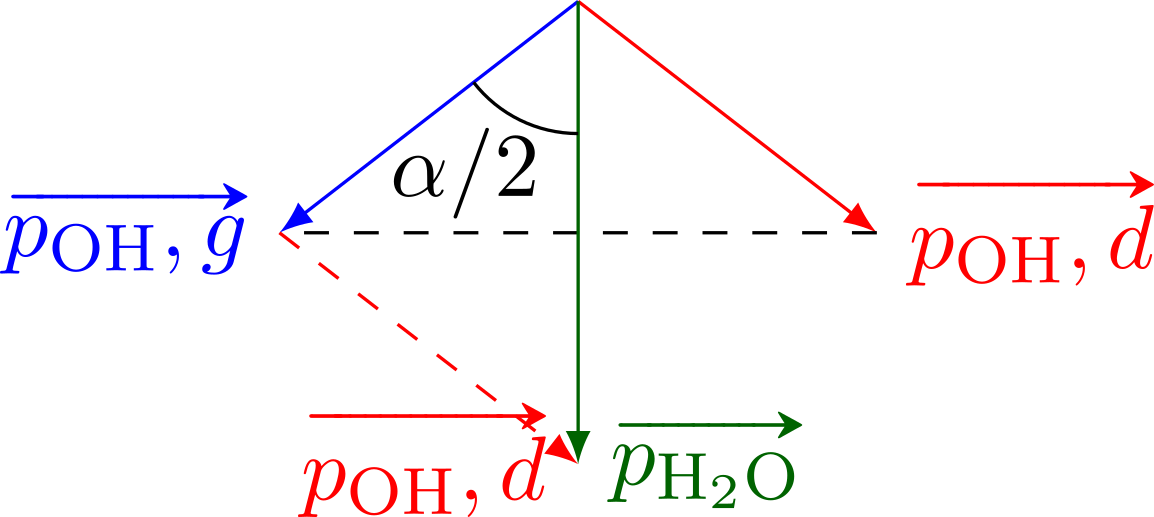
\includegraphics[scale=.8]{pH2O}}}$
			\end{center}
			\tcblower
			\begin{gather*}
				\beforetext{On trouve}
				\cos(\frac{\a}{2}) = \frac{\mu_{\ce{H2O}}/2}{\mu_{\ce{OH}}}
				\\\Lra
				\boxed{
					\mu_{\ce{H2O}} \stm[-1]{=}
					2\mu_{\ce{OH}}\cos(\a/2) \stm[-1]{=}
					\SI{1.85}{D}
				}
			\end{gather*}
		\end{isd}
		\vspace{-15pt}
	}

	\QR[4\hspace{-15pt}]{%
		Écrire la norme du moment dipolaire $\norm{\muf_{\ce{O-H}}}$ en fonction des
		données. Déterminer la charge partielle portée par l'hydrogène. L'exprimer
		en \si{C} puis en fraction de $e$ la charge élémentaire. Quel est le
		pourcentage d'ionicité de la liaison~?
	}{%
		\vspace{-15pt}
		\begin{gather*}
			\beforetext{On a}
			\norm{\muf_{\ce{O-H}}} \stm[-1]{=} q \ell_{\ce{O-H}}
			\Lra
			\boxed{q = \frac{\mu_{\ce{O-H}}}{\ell_{\ce{O-H}}}}
			\qav
			\left\{
			\begin{array}{rcl}
				\mu_{\ce{O-H}}  & = & \SI{1.51}{D} = \SI{5.03e-30}{C.m}
				\\
				\ell_{\ce{O-H}} & = & \SI{95.84e-12}{m}
			\end{array}
			\right.\\
			\AN
			\xul{
				q \stm[-1]{=} \SI{5.24e-20}{C} \stm[-1]{=} \num{0.33}e
			}
			\\
			\beforetext{Par définition,}
			\boxed{\delta \stm[-1]{=} \frac{q}{e}}
			\Lra
			\xul{\delta = \num{0.33}}
		\end{gather*}
	}

	\QR[6\hspace{-15pt}]{%
		Qu'est-ce que la liaison hydrogène et quelles sont les conditions pour
		qu'elle existe~? Quel type de solvant est l'eau~? Citer
		des conséquences de ces propriétés.
	}{%
		Une \textbf{liaison hydrogène} s'établit entre un atome d'\textbf{hydrogène
			porté par un atome très électronégatif} \pt{1} (\ce{N}, \ce{O} ou \ce{F}) et
		un autre atome \ce{B} également très électronégatif, porteur d'au moins un
		\textbf{doublet non-liant} \pt{1} et neutre.
		\smallbreak
		L'eau est un solvant \textbf{polaire et protique} \pt{1}. De plus il est
		\textbf{très dispersant} \pt{1} car $\ep_r$ est élevée.
		\smallbreak
		L'eau est donc miscible \pt{1} avec des solvants polaires et protiques , et
		solubilise \pt{1} fortement tous les solides ioniques.
	}
\end{blocQR}

\begin{blocQR}
	\item
	\QR[2]{%
		Indiquer ce qu'on appelle les interactions de \textsc{Van der Waals}.
		Nommez les interactions possibles et préciser leur nature.
	}{%
		Les interactions de \textsc{Van der Waals} sont des interactions attractives
		\pt{1} dues à la force électrostatique intermoléculaires.
		\smallbreak
		On peut distinguer les contributions des effets \textsc{Keesom},
		\textsc{Debye} et \textsc{London} selon si ces interactions ont lieu entre
		deux molécules polaires, 1 polaire 1 polarisable, ou deux molécules
		polarisables respectivement. \pt{1}
	}

	\QR[3\hspace{-15pt}]{%
	Donnez un ordre de grandeur des énergies de liaison des trois grands types de
	liaison chimique possible (pas que \textsc{Van der Waals}).
	}{%
	\vspace{-15pt}
	\[
		\stm{
		\underbracket[1pt]{E\ind{covalente}}_{\approx\SI{500}{kJ.mol^{-1}}}
		}
		\gg
		\stm{
		\underbracket[1pt]{E\ind{LH}}_{\approx\SI{20}{kJ.mol^{-1}}}
		}
		\gg
		\stm{
		\underbracket[1pt]{E\ind{VdW}}_{\approx\SI{1}{kJ.mol^{-1}}}
		}
	\]
	}

	\QR[3\hspace{-15pt}]{%
		Selon vous le diiode est-il soluble dans l'eau~? Dans le cyclohexane~?
	}{%
		Le diiode est une molécule \textbf{apolaire et aprotique} \pt{1}. Il est
		donc peu soluble dans l'eau \pt{1}.
		\smallbreak
		Le cyclohexane étant une molécule \textbf{apolaire et aprotique}, le diiode
		ayant les mêmes caractéristiques, il sera soluble dans le cyclohexane
		\pt{1}.
	}

\end{blocQR}
% \resetQ
% \chapter{Sujet 1\siCorrige{\!\!-- corrigé}}
%
% \subimport{/home/nora/Documents/Enseignement/Prepa/bpep/exercices/DS/molecules_lewis/}{sujet.tex}
%
%
% \resetQ
% \chapter{Sujet 2\siCorrige{\!\!-- corrigé}}
%
% \subimport{/home/nora/Documents/Enseignement/Prepa/bpep/exercices/DS/alcools_liaison_H/}{sujet.tex}
\end{document}
